% Options for packages loaded elsewhere
\PassOptionsToPackage{unicode}{hyperref}
\PassOptionsToPackage{hyphens}{url}
\PassOptionsToPackage{dvipsnames,svgnames,x11names}{xcolor}
%
\documentclass[
  letterpaper,
  DIV=11,
  numbers=noendperiod]{scrartcl}

\usepackage{amsmath,amssymb}
\usepackage{iftex}
\ifPDFTeX
  \usepackage[T1]{fontenc}
  \usepackage[utf8]{inputenc}
  \usepackage{textcomp} % provide euro and other symbols
\else % if luatex or xetex
  \usepackage{unicode-math}
  \defaultfontfeatures{Scale=MatchLowercase}
  \defaultfontfeatures[\rmfamily]{Ligatures=TeX,Scale=1}
\fi
\usepackage{lmodern}
\ifPDFTeX\else  
    % xetex/luatex font selection
  \setmainfont[]{Inter}
  \setsansfont[]{Inter}
  \setmathfont[]{Fira Math}
\fi
% Use upquote if available, for straight quotes in verbatim environments
\IfFileExists{upquote.sty}{\usepackage{upquote}}{}
\IfFileExists{microtype.sty}{% use microtype if available
  \usepackage[]{microtype}
  \UseMicrotypeSet[protrusion]{basicmath} % disable protrusion for tt fonts
}{}
\makeatletter
\@ifundefined{KOMAClassName}{% if non-KOMA class
  \IfFileExists{parskip.sty}{%
    \usepackage{parskip}
  }{% else
    \setlength{\parindent}{0pt}
    \setlength{\parskip}{6pt plus 2pt minus 1pt}}
}{% if KOMA class
  \KOMAoptions{parskip=half}}
\makeatother
\usepackage{xcolor}
\usepackage{soul}
\setlength{\emergencystretch}{3em} % prevent overfull lines
\setcounter{secnumdepth}{5}
% Make \paragraph and \subparagraph free-standing
\ifx\paragraph\undefined\else
  \let\oldparagraph\paragraph
  \renewcommand{\paragraph}[1]{\oldparagraph{#1}\mbox{}}
\fi
\ifx\subparagraph\undefined\else
  \let\oldsubparagraph\subparagraph
  \renewcommand{\subparagraph}[1]{\oldsubparagraph{#1}\mbox{}}
\fi


\providecommand{\tightlist}{%
  \setlength{\itemsep}{0pt}\setlength{\parskip}{0pt}}\usepackage{longtable,booktabs,array}
\usepackage{calc} % for calculating minipage widths
% Correct order of tables after \paragraph or \subparagraph
\usepackage{etoolbox}
\makeatletter
\patchcmd\longtable{\par}{\if@noskipsec\mbox{}\fi\par}{}{}
\makeatother
% Allow footnotes in longtable head/foot
\IfFileExists{footnotehyper.sty}{\usepackage{footnotehyper}}{\usepackage{footnote}}
\makesavenoteenv{longtable}
\usepackage{graphicx}
\makeatletter
\def\maxwidth{\ifdim\Gin@nat@width>\linewidth\linewidth\else\Gin@nat@width\fi}
\def\maxheight{\ifdim\Gin@nat@height>\textheight\textheight\else\Gin@nat@height\fi}
\makeatother
% Scale images if necessary, so that they will not overflow the page
% margins by default, and it is still possible to overwrite the defaults
% using explicit options in \includegraphics[width, height, ...]{}
\setkeys{Gin}{width=\maxwidth,height=\maxheight,keepaspectratio}
% Set default figure placement to htbp
\makeatletter
\def\fps@figure{htbp}
\makeatother

\usepackage{amsmath, xparse}
\usepackage{fancyvrb, fvextra}
\usepackage{amssymb}
\usepackage{graphicx}
\usepackage{bm}
\usepackage{svg}
\usepackage{listings}
\usepackage{tikz}
\usepackage{multicol}
\usepackage{xifthen}
\DefineVerbatimEnvironment{Highlighting}{Verbatim}{breaklines,commandchars=\\\{\}}
\lstset{basicstyle=\ttfamily\footnotesize,breaklines=true}
\newcommand\encircle[1]{%
  \tikz[baseline=(X.base)]
    \node (X) [draw, shape=circle, inner sep=0] {\strut #1};}
\KOMAoption{captions}{tableheading}
\makeatletter
\makeatother
\makeatletter
\makeatother
\makeatletter
\@ifpackageloaded{caption}{}{\usepackage{caption}}
\AtBeginDocument{%
\ifdefined\contentsname
  \renewcommand*\contentsname{Table of contents}
\else
  \newcommand\contentsname{Table of contents}
\fi
\ifdefined\listfigurename
  \renewcommand*\listfigurename{List of Figures}
\else
  \newcommand\listfigurename{List of Figures}
\fi
\ifdefined\listtablename
  \renewcommand*\listtablename{List of Tables}
\else
  \newcommand\listtablename{List of Tables}
\fi
\ifdefined\figurename
  \renewcommand*\figurename{Figure}
\else
  \newcommand\figurename{Figure}
\fi
\ifdefined\tablename
  \renewcommand*\tablename{Table}
\else
  \newcommand\tablename{Table}
\fi
}
\@ifpackageloaded{float}{}{\usepackage{float}}
\floatstyle{ruled}
\@ifundefined{c@chapter}{\newfloat{codelisting}{h}{lop}}{\newfloat{codelisting}{h}{lop}[chapter]}
\floatname{codelisting}{Listing}
\newcommand*\listoflistings{\listof{codelisting}{List of Listings}}
\makeatother
\makeatletter
\@ifpackageloaded{caption}{}{\usepackage{caption}}
\@ifpackageloaded{subcaption}{}{\usepackage{subcaption}}
\makeatother
\makeatletter
\@ifpackageloaded{tcolorbox}{}{\usepackage[skins,breakable]{tcolorbox}}
\makeatother
\makeatletter
\@ifundefined{shadecolor}{\definecolor{shadecolor}{rgb}{.97, .97, .97}}
\makeatother
\makeatletter
\makeatother
\makeatletter
\makeatother
\ifLuaTeX
  \usepackage{selnolig}  % disable illegal ligatures
\fi
\IfFileExists{bookmark.sty}{\usepackage{bookmark}}{\usepackage{hyperref}}
\IfFileExists{xurl.sty}{\usepackage{xurl}}{} % add URL line breaks if available
\urlstyle{same} % disable monospaced font for URLs
\hypersetup{
  colorlinks=true,
  linkcolor={blue},
  filecolor={Maroon},
  citecolor={Blue},
  urlcolor={Blue},
  pdfcreator={LaTeX via pandoc}}

\author{}
\date{}

\begin{document}
\begin{titlepage}

    \newcommand{\HRule}{\rule{\linewidth}{0.5mm}}
    
    \center
    
    \vspace{10cm}

    \textsc{\LARGE Gwinnett School of Math, Science, and Technology }\\[0.3cm]
    
    \vspace{0.5cm}

    \HRule \\[0.4cm]
    { \huge \bfseries AP Physics: Mechanics/Electricity \& Magnetism Notes}\\[0.03cm]
    \HRule \\[1.5cm]
    
    \begin{minipage}{0.4\textwidth}
    \begin{flushleft} \Large
    Anish Goyal \\3rd/4th Period
    \end{flushleft}
    \end{minipage}
    ~
    \begin{minipage}{0.4\textwidth}
    \begin{flushright} \Large
    Jeffrey Burmester\\Educator
    \end{flushright}
    \end{minipage}\\[1cm]
    
    {\huge 2023-2024}\\[1cm]
    
    
\includegraphics{img/logo.png}\\
    \vfill
    \end{titlepage}
\newpage

\ifdefined\Shaded\renewenvironment{Shaded}{\begin{tcolorbox}[frame hidden, interior hidden, boxrule=0pt, enhanced, sharp corners, breakable, borderline west={3pt}{0pt}{shadecolor}]}{\end{tcolorbox}}\fi

\renewcommand*\contentsname{Table of Contents}
{
\hypersetup{linkcolor=}
\setcounter{tocdepth}{4}
\tableofcontents
}
\newpage{}

\hypertarget{kinematics}{%
\section{Kinematics}\label{kinematics}}

\hypertarget{variables}{%
\subsection{Variables}\label{variables}}

\hypertarget{position}{%
\subsubsection{Position}\label{position}}

\begin{itemize}
\tightlist
\item
  Typically given by the variable \(x\)
\end{itemize}

\hypertarget{time}{%
\subsubsection{Time}\label{time}}

\begin{itemize}
\tightlist
\item
  Typically given by the variables \(t\)
\end{itemize}

\hypertarget{displacement}{%
\subsubsection{Displacement}\label{displacement}}

\begin{itemize}
\tightlist
\item
  Defined as the change in position (\(X_f - X_i\))
\item
  Given by the variable \(\Delta x\)
\end{itemize}

\hypertarget{distance}{%
\subsubsection{Distance}\label{distance}}

\begin{itemize}
\tightlist
\item
  You have to take the magnitude of vectors for every time you change
  position
\item
  \(S = |x_2 - x_1| + |x_1 - x_0| + ...\)
\end{itemize}

\hypertarget{average-velocity}{%
\subsubsection{Average Velocity}\label{average-velocity}}

\begin{itemize}
\tightlist
\item
  Defined as the change in displacement over time
\item
  \(\frac{\Delta x}{\Delta t} = V_\text{avg} = \bar{V}\)
\end{itemize}

\hypertarget{velocity}{%
\subsubsection{Velocity}\label{velocity}}

\begin{itemize}
\tightlist
\item
  Defined as the change in displacement as time approaches 0
\item
  \(\lim_{\Delta t \to 0} \frac{\Delta x}{\Delta t} = \frac{dx}{dt} = V\)
\end{itemize}

\hypertarget{average-acceleration}{%
\subsubsection{Average Acceleration}\label{average-acceleration}}

\begin{itemize}
\tightlist
\item
  Defined as the change in velocity over time
\item
  \(\frac{\Delta V}{\Delta t} = A_\text{avg} = \bar{A}\)
\end{itemize}

\hypertarget{acceleration}{%
\subsubsection{Acceleration}\label{acceleration}}

\begin{itemize}
\tightlist
\item
  Defined as the change in velocity as time approaches 0
\item
  \(a = \lim_{\Delta t \to 0} \frac{\Delta V}{\Delta t} = \frac{dV}{dt} = \frac{d^2x}{dt^2}\)
\end{itemize}

\hypertarget{speed}{%
\subsubsection{Speed}\label{speed}}

\begin{itemize}
\tightlist
\item
  \(\text{Speed} = \frac{S}{t}\)
\item
  Alternatively, when referring to vectors:
  \(\text{Speed} = ||\vec{V}||\)
\end{itemize}

\hypertarget{velocity-and-position-definitions-0803-homework}{%
\subsection{Velocity and Position Definitions (08/03
Homework)}\label{velocity-and-position-definitions-0803-homework}}

\hypertarget{problem-1}{%
\subsubsection{Problem 1}\label{problem-1}}

The position versus time for a certain particle moving along the x axis
is shown in the figure below. Find the average velocity in the following
time intervals.

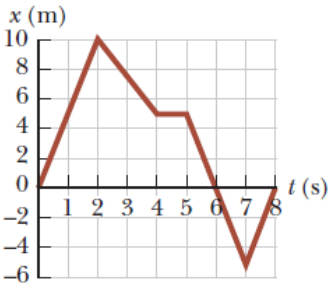
\includegraphics{img/Kinematics Velocity and Position HW/problem1.png}

\begin{enumerate}
\def\labelenumi{(\alph{enumi})}
\tightlist
\item
  0 to 2s
\end{enumerate}

\begin{itemize}
\tightlist
\item
  \(\frac{10-0}{2-0} = \frac{10}{2} = 5.000\) m/s
\end{itemize}

\begin{enumerate}
\def\labelenumi{(\alph{enumi})}
\setcounter{enumi}{1}
\tightlist
\item
  0 to 4s
\end{enumerate}

\begin{itemize}
\tightlist
\item
  \(\frac{5-0}{4-0}=\frac{5}{4}=1.250\) m/s
\end{itemize}

\begin{enumerate}
\def\labelenumi{(\alph{enumi})}
\setcounter{enumi}{2}
\tightlist
\item
  2 to 6s
\end{enumerate}

\begin{itemize}
\tightlist
\item
  \(\frac{0-10}{6-2}=\frac{-10}{4}=-2.500\) m/s
\end{itemize}

\begin{enumerate}
\def\labelenumi{(\alph{enumi})}
\setcounter{enumi}{3}
\tightlist
\item
  1 to 7s
\end{enumerate}

\begin{itemize}
\tightlist
\item
  \(\frac{-5-5}{7-1}=\frac{-10}{6}=-1.667\) m/s
\end{itemize}

\begin{enumerate}
\def\labelenumi{(\alph{enumi})}
\setcounter{enumi}{4}
\tightlist
\item
  0 to 7s
\end{enumerate}

\begin{itemize}
\tightlist
\item
  \(\frac{-5-0}{7-0}=\frac{-5}{7}=-0.714\) s
\end{itemize}

\newpage{}

\hypertarget{problem-2}{%
\subsubsection{Problem 2}\label{problem-2}}

A person walks first at a constant speed of \(4.80\) m/s along a
straight line from point \encircle{$A$} to point \encircle{$B$} and then
back along the line from \encircle{$B$} to \encircle{$A$} at a constant
speed of \(2.90\) m/s.

\begin{enumerate}
\def\labelenumi{(\alph{enumi})}
\tightlist
\item
  What is her average speed over the entire trip?
\end{enumerate}

\begin{align*}
\text{Average speed} &= \frac{d_{AB}+d_{BA}}{t_{AB}+t_{BA}} \\
d &= d_{AB} = d_{BA} \\
t_{AB} &= \frac{d}{V_{AB}} \\
t{BA} &= \frac{d}{V_{BA}} \\
\therefore \text{ Average speed} &= \frac{d+d}{\frac{d}{V_{AB}}+\frac{d}{V_{BA}}} \\
&= \frac{2d(V_{AB})(V_{BA})}{2d} \\
&= \frac{2(V_{AB})(V_{BA})}{V_{AB}+V_{BA}} \\
&= 2\left[\frac{(4.80)(2.90)}{4.80+2.90}\right] \\
&= 3.615
\end{align*}

\begin{enumerate}
\def\labelenumi{(\alph{enumi})}
\setcounter{enumi}{1}
\tightlist
\item
  What is her average velocity over the entire trip?
\end{enumerate}

\begin{itemize}
\tightlist
\item
  Since her displacement is 0, her average velocity is also 0.
\end{itemize}

\newpage{}

\hypertarget{problem-3}{%
\subsubsection{Problem 3}\label{problem-3}}

A position-time graph for a particle moving along the x axis is shown in
the figure below.

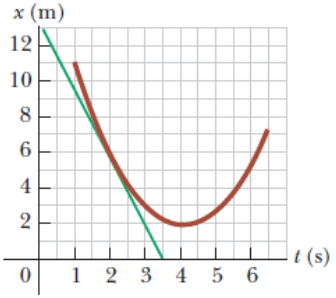
\includegraphics{img/Kinematics Velocity and Position HW/problem3.png}

\begin{enumerate}
\def\labelenumi{(\alph{enumi})}
\tightlist
\item
  Find the average velocity in the time interval \(t = 2.00\) s to
  \(t = 3.50\) s.
\end{enumerate}

\begin{itemize}
\tightlist
\item
  \(\frac{2-6}{3.5-2}=\frac{-4}{1.5}=-2.667\) m/s
\end{itemize}

\begin{enumerate}
\def\labelenumi{(\alph{enumi})}
\setcounter{enumi}{1}
\tightlist
\item
  Determine the instantaneous velocity at \(t = 2\) s (where the tangent
  line touches the curve) by measuring the slope of the tangent line
  shown in the graph.
\end{enumerate}

\begin{itemize}
\tightlist
\item
  \(\frac{2-12}{3.5-0} = \frac{-10}{3.5} = -3.714\) m/s
\end{itemize}

\begin{enumerate}
\def\labelenumi{(\alph{enumi})}
\setcounter{enumi}{2}
\tightlist
\item
  At what value of \(t\) is the velocity zero?
\end{enumerate}

\begin{itemize}
\tightlist
\item
  4.000 s
\end{itemize}

\newpage{}

\hypertarget{problem-4}{%
\subsubsection{Problem 4}\label{problem-4}}

A person takes a trip, driving with a constant speed of \(91.5\) km/h,
except for a \(24.0\)-min rest stop. The person's average speed is
\(71.6\) km/h.

\begin{enumerate}
\def\labelenumi{(\alph{enumi})}
\tightlist
\item
  How much time is spent on the trip? \begin{align*}
  \bar{V} &= \frac{(\text{Time driving})*V_\text{driving}}{\text{Total time}} \\
  71.6 &= \cfrac{(t-\frac{24}{60})\cdot 91.5}{t} \\
  71.6t &= (t-\frac{24}{60})\cdot 91.5 \\
  \frac{71.6}{91.5}t &= t-\frac{24}{60} \\
  \frac{71.6}{91.5}t - t &= -\frac{24}{60} \\
  \frac{71.6}{91.5}t - \frac{91.5}{91.5}t &= -\frac{24}{60} \\
  -\frac{19.9}{91.5}t &= -\frac{24}{60} \\
  t &= -\frac{24}{60}\cdot -\frac{91.5}{19.9} \\
  t &= 1.839 \text{ hours}
  \end{align*}
\item
  How far does the person travel?
\end{enumerate}

\begin{itemize}
\tightlist
\item
  \(d = \bar{V}\cdot t = (71.6)(1.839) = 131.6\) km
\end{itemize}

\newpage{}

\hypertarget{derivative-relationships}{%
\subsection{Derivative Relationships}\label{derivative-relationships}}

\hypertarget{acceleration-and-velocity}{%
\subsubsection{Acceleration and
Velocity}\label{acceleration-and-velocity}}

\begin{itemize}
\tightlist
\item
  \(a = \frac{dV}{dt}\)
\item
  \(V = \frac{dx}{dt}\)
\item
  \(V = at + V_0\)
\end{itemize}

\hypertarget{acceleration-and-position}{%
\subsubsection{Acceleration and
Position}\label{acceleration-and-position}}

\begin{itemize}
\tightlist
\item
  \(V = \frac{dx}{dt}\)
\item
  \(x = \frac{1}{2}at^2 + V_0t\)
\end{itemize}

\emph{If initial time or position is not zero:}

\begin{itemize}
\tightlist
\item
  \(x-x_0 = V_0(t-t_0) + \frac{1}{2}a(t-t_0)^2\)
\end{itemize}

\hypertarget{given-x4t4---6t-find-a-when-t2.}{%
\subsubsection{\texorpdfstring{Given \(x=4t^4 - 6t\), find \(a\) when
\(t=2\).}{Given x=4t\^{}4 - 6t, find a when t=2.}}\label{given-x4t4---6t-find-a-when-t2.}}

\begin{align*}
\frac{dx}{dt} &= 16t^3 - 6 \\
\frac{d^2x}{dt^2} &= 48t^2 \\
a &= 48(2)^2 \\
a &= 192
\end{align*}

\newpage{}

\hypertarget{practice-with-1-d-kinematic-equations-moderate}{%
\subsection{Practice with 1-D Kinematic Equations
(moderate)}\label{practice-with-1-d-kinematic-equations-moderate}}

\hypertarget{problem-1-1}{%
\subsubsection{Problem 1}\label{problem-1-1}}

A world-class sprinter can burst out of the blocks to essentially top
speed (of about \(11.5\) m/s) in the first \(15.0\)m of the race. What
is the average acceleration of this sprinter and how long does it take
her to reach that speed (she accelerates uniformly)?

\hypertarget{problem-2-1}{%
\subsubsection{Problem 2}\label{problem-2-1}}

A car slows down from a speed of \(25.0\)m/s to rest in \(5.0\)s. How
far did it travel in that time?

\hypertarget{problem-3-1}{%
\subsubsection{Problem 3}\label{problem-3-1}}

In coming to a stop, a car leaves skid marks 80m long on the highway.
Assuming a deceleration of \(7.00 \text{m/s}^2\), estimate the speed of
the car just before braking.

\hypertarget{problem-4-1}{%
\subsubsection{Problem 4}\label{problem-4-1}}

A car traveling \(45\)km/h slows down at a constant
\(0.50 \text{m/s}^2\) just by ``letting up on the gas.'' Calculate:

\begin{enumerate}
\def\labelenumi{(\alph{enumi})}
\tightlist
\item
  the distance the car coasts before it stops
\item
  the time it takes to stop
\item
  the distance it travels during the first and fifth seconds
\end{enumerate}

\hypertarget{problem-5}{%
\subsubsection{Problem 5}\label{problem-5}}

A car traveling at \(90\)km/h strikes a tree. The front end of the car
compresses and the driver comes to rest after traveling \(0.80\)m. What
was the average acceleration of the driver during the collision? Express
the answer in terms of ``g's,'' where
\(1.00\text{g} = 9.80 \text{m/s}^2\)

\hypertarget{problem-6}{%
\subsubsection{Problem 6}\label{problem-6}}

Determine the stopping distances for an automobile with ana initial
speed of 90km/h and human reaction time of 1.0s:

\begin{enumerate}
\def\labelenumi{(\alph{enumi})}
\tightlist
\item
  for \(a =-4.0 \text{m/s}^2\)
\item
  for \(a = -8.0 \text{m/s}^2\)
\end{enumerate}

\hypertarget{acceleration-definitions-0804-homework}{%
\subsection{Acceleration Definitions (08/04
Homework)}\label{acceleration-definitions-0804-homework}}

\hypertarget{problem-1-2}{%
\subsubsection{Problem 1}\label{problem-1-2}}

A \(48.0\) g Super Ball traveling at \(29.0\) m/s bounces off a brick
wall and rebounds at \(18.0\) m/s. A high-speed camera records this
event. If the ball is in contact with the wall for \(4.05\) ms, what is
the magnitude of the average acceleration of the ball during this time
interval?

\begin{itemize}
\tightlist
\item
  \(a = \left|\frac{-18-29}{0.00405} = 11604.938\right|\) m/s\(^2\)
\end{itemize}

\newpage{}

\hypertarget{problem-2-2}{%
\subsubsection{Problem 2}\label{problem-2-2}}

A child rolls a marble on a bent track that is 100 cm long as shown in
the figure below. We use \(x\) to represent the position of the marble
along the track. On the horizontal sections from \(x=0\) to \(x=20\) cm
and from \(x=40\) to \(x=60\) cm, the marble rolls with constant speed.
On the sloping sections, the marble's speed changes steadily. At the
places where the slope changes, the marble stays on the track and does
not undergo any sudden changes in speed. The child gives the marble some
initial speed at \(x=0\) and \(t=0\) and then watches it roll to
\(x=90\) cm, where it turns around, eventually returning to \(x=0\) with
the same speed with which the child released it. Prepare graphs of \(x\)
versus \(t, v_x\) versus \(t\), and \(a_x\) versus \(t\), with their
time axes identical, to show the motion of the marble. You will not be
able to place any numbers other than zero on the horizontal axis or on
the velocity and acceleration axes, but show the correct graph shapes.

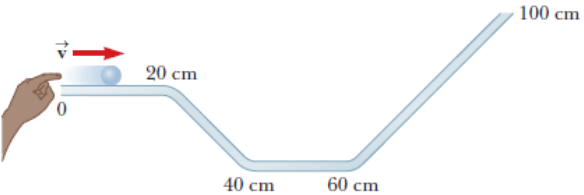
\includegraphics{img/Acceleration Definitions HW/problem1.png}

\newpage{}

\begin{figure}[!htb]
   \begin{minipage}{0.48\textwidth}
     \centering
     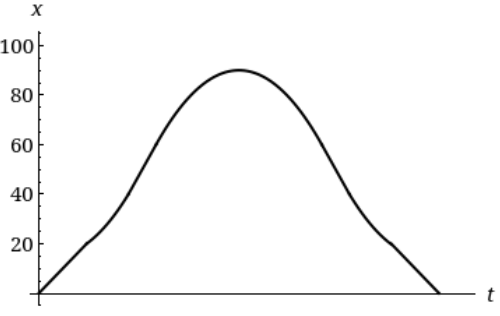
\includegraphics[width=\linewidth]{img/Acceleration Definitions HW/xversust.png}
     \caption*{$x$ versus $t$}
   \end{minipage}\hfill
   \begin{minipage}{0.48\textwidth}
     \centering
     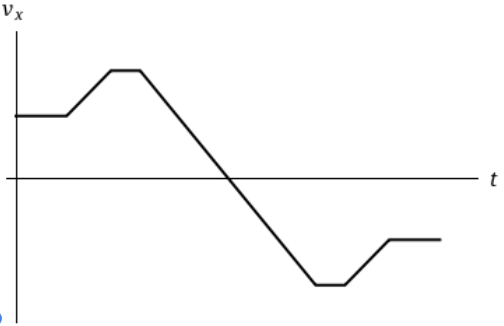
\includegraphics[width=\linewidth]{img/Acceleration Definitions HW/vxversust.png}
     \caption*{$V_x$ versus $t$}
   \end{minipage}
\end{figure}

\begin{figure}[!htb]
\begin{center}
   \begin{minipage}{0.48\textwidth}
     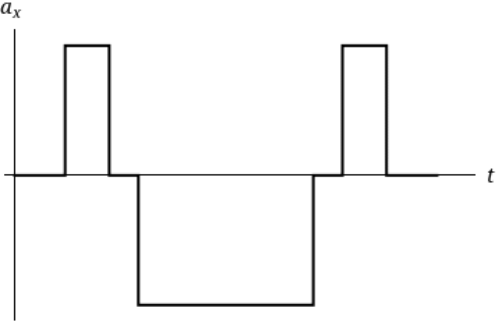
\includegraphics[width=\linewidth]{img/Acceleration Definitions HW/axversust.png}
     \caption*{$a_x$ versus $t$}
  \end{minipage}\hfill
\end{center}
\end{figure}

\newpage{}

\hypertarget{problem-3-2}{%
\subsubsection{Problem 3}\label{problem-3-2}}

A particle starts from rest and accelerates as shown in the figure
below.

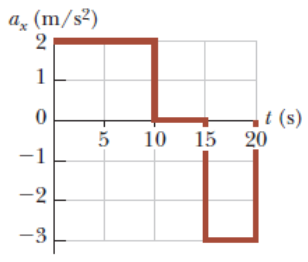
\includegraphics{img/Acceleration Definitions HW/problem3.png}

\begin{enumerate}
\def\labelenumi{(\alph{enumi})}
\tightlist
\item
  Determine the particle's speed at \(t = 10.0\) s.
\end{enumerate}

\begin{itemize}
\tightlist
\item
  \(\int_0^{10} a \ \mathrm{d}t = 10 \cdot 2 = 20\) m/s
\end{itemize}

\begin{enumerate}
\def\labelenumi{(\alph{enumi})}
\setcounter{enumi}{1}
\tightlist
\item
  Determine the particle's speed at \(t = 20.0\) s?
\end{enumerate}

\begin{itemize}
\tightlist
\item
  \(\int_0^{20} a \ \mathrm{d}t = 10 \cdot 2 + 5 \cdot (-3) = 20 - 15 = 5\)
  m/s
\end{itemize}

\begin{enumerate}
\def\labelenumi{(\alph{enumi})}
\setcounter{enumi}{2}
\tightlist
\item
  Determine the distance traveled in the first \(20.0\) s. (Enter your
  answer to one decimal places.) \begin{align*}
  \Delta x \text{ from 0-10 seconds: }\frac{1}{2} \cdot 2 \cdot 10^2 &= 100 \\
  \Delta x \text{ from 10-15 seconds: }20 \cdot 5 &= 100 \\
  \Delta x \text{ from 15-20 seconds: } \frac{1}{2} \cdot -3 \cdot 5^2 + 20 \cdot 5 &= 62.5 \\
  \therefore \Delta x &= 262.5 \text{ m}
  \end{align*}
\end{enumerate}

\hypertarget{problem-4-2}{%
\subsubsection{Problem 4}\label{problem-4-2}}

An object moves along the x axis according to the equation
\(x = 3.25t^2 − 2.00t + 3.00\), where \(x\) is in meters and \(t\) is in
seconds.

\begin{enumerate}
\def\labelenumi{(\alph{enumi})}
\tightlist
\item
  Determine the average speed between \(t = 1.70\) s and \(t = 3.30\) s.
\end{enumerate}

\begin{itemize}
\tightlist
\item
  \(\bar{V} = \frac{x(3.30)-x(1.70)}{t_1-t_0} = \frac{(3.25(3.30)^2-2(3.30)+3) - (3.25(1.70)^2-2(1.70)+3)}{3.30-1.70} = 14.25\)
  m/s
\end{itemize}

\begin{enumerate}
\def\labelenumi{(\alph{enumi})}
\setcounter{enumi}{1}
\tightlist
\item
  Determine the instantaneous speed at \(t = 1.70\) s.
\end{enumerate}

\begin{itemize}
\tightlist
\item
  \(V = \frac{dx}{dt} = 6.5(1.7)-2 = 9.05\) m/s
\end{itemize}

\begin{enumerate}
\def\labelenumi{(\alph{enumi})}
\setcounter{enumi}{2}
\tightlist
\item
  Determine the instantaneous speed at \(t = 3.30\) s.
\end{enumerate}

\begin{itemize}
\tightlist
\item
  \(V = \frac{dx}{dt} = 2(3.25)(3.3)-2 = 19.45\) m/s
\end{itemize}

\begin{enumerate}
\def\labelenumi{(\alph{enumi})}
\setcounter{enumi}{3}
\tightlist
\item
  Determine the average acceleration between \(t = 1.70 s\) and
  \(t = 3.30\) s.
\end{enumerate}

\begin{itemize}
\tightlist
\item
  \(\bar{a} = \frac{V(3.30)-V(1.70)}{t_1-t_0} = \frac{(2(3.25)(3.30)-2)-(2(3.25)(1.70)-2)}{3.30-1.70} = 6.5\)
  m/s\(^2\)
\end{itemize}

\begin{enumerate}
\def\labelenumi{(\alph{enumi})}
\setcounter{enumi}{4}
\tightlist
\item
  Determine the instantaneous acceleration at \(t = 1.70\) s.
\end{enumerate}

\begin{itemize}
\tightlist
\item
  \(a = \frac{dV}{dt} = 2(3.25) = 6.5\) m/s\(^2\)
\end{itemize}

\begin{enumerate}
\def\labelenumi{(\alph{enumi})}
\setcounter{enumi}{5}
\tightlist
\item
  Determine the instantaneous acceleration at \(t = 3.30\) s.
\end{enumerate}

\begin{itemize}
\tightlist
\item
  \(a = \frac{dV}{dt} = 2(3.25) = 6.5\) m/s\(^2\)
\end{itemize}

\begin{enumerate}
\def\labelenumi{(\alph{enumi})}
\setcounter{enumi}{6}
\tightlist
\item
  At what time is the object at rest?
\end{enumerate}

\begin{itemize}
\tightlist
\item
  0 = \(6.5t-2 \implies 0.308\) s
\end{itemize}

\newpage{}

\hypertarget{velocity-acceleration-relationships}{%
\subsection{Velocity-Acceleration
Relationships}\label{velocity-acceleration-relationships}}

\begin{itemize}
\tightlist
\item
  If acceleration is constant, \(\frac{\mathrm{d}a}{\mathrm{d}t} = 0\)

  \begin{itemize}
  \tightlist
  \item
    And as long as acceleration remains constant, and \(V_0\) and
    \(t_0\) are 0, \(\bar{V} = \frac{1}{2}(V_0 + V_f)\)
  \end{itemize}
\item
  If acceleration is constant, but either \(V_0\) or \(t_0\) are not 0,
  \(X = V_0t + \frac{1}{2}V_ft-\frac{1}{2}V_0t_0\)
\end{itemize}

\hypertarget{phab-four}{%
\subsubsection{Phab Four}\label{phab-four}}

\begin{enumerate}
\def\labelenumi{\arabic{enumi}.}
\tightlist
\item
  \(V_f = V_0 + at\)
\item
  \(t = \frac{1}{2}t(V_0 + V_f)\)
\item
  \(x = V_0t + \frac{1}{2}at^2\)
\item
  \(V_f^2 = V_0^2 + 2ax\)
\end{enumerate}

\begin{longtable}[]{@{}
  >{\raggedright\arraybackslash}p{(\columnwidth - 10\tabcolsep) * \real{0.5397}}
  >{\raggedright\arraybackslash}p{(\columnwidth - 10\tabcolsep) * \real{0.1111}}
  >{\raggedright\arraybackslash}p{(\columnwidth - 10\tabcolsep) * \real{0.1111}}
  >{\raggedright\arraybackslash}p{(\columnwidth - 10\tabcolsep) * \real{0.0794}}
  >{\raggedright\arraybackslash}p{(\columnwidth - 10\tabcolsep) * \real{0.0794}}
  >{\raggedright\arraybackslash}p{(\columnwidth - 10\tabcolsep) * \real{0.0794}}@{}}
\toprule\noalign{}
\begin{minipage}[b]{\linewidth}\raggedright
Phab Four
\end{minipage} & \begin{minipage}[b]{\linewidth}\raggedright
\texttt{V\_0}
\end{minipage} & \begin{minipage}[b]{\linewidth}\raggedright
\texttt{V\_f}
\end{minipage} & \begin{minipage}[b]{\linewidth}\raggedright
\texttt{a}
\end{minipage} & \begin{minipage}[b]{\linewidth}\raggedright
\texttt{t}
\end{minipage} & \begin{minipage}[b]{\linewidth}\raggedright
\texttt{x}
\end{minipage} \\
\midrule\noalign{}
\endhead
\bottomrule\noalign{}
\endlastfoot
\(V_f = V_0 + at\) & \checkmark & \checkmark & \checkmark & \checkmark
& \\
\(t = \frac{1}{2}(V_0 + V_f)\) & \checkmark & \checkmark & & \checkmark
& \\
\(x = V_0t + \frac{1}{2}at^2\) & \checkmark & & \checkmark & \checkmark
& \checkmark \\
\(V_f^2 = V_0^2 + 2ax\) & \checkmark & \checkmark & \checkmark & &
\checkmark \\
\end{longtable}

\hypertarget{what-if-v_0-isnt-given}{%
\subsubsection{\texorpdfstring{What if \(V_0\) isn't
given?}{What if V\_0 isn't given?}}\label{what-if-v_0-isnt-given}}

\begin{itemize}
\tightlist
\item
  Simply use the equation \(x = V_ft-\frac{1}{2}at^2\)

  \begin{itemize}
  \tightlist
  \item
    This will rarely show up, if ever.
  \end{itemize}
\end{itemize}

\hypertarget{what-if-time-andor-starting-distance-are-not-0}{%
\subsubsection{What if time and/or starting distance are not
0?}\label{what-if-time-andor-starting-distance-are-not-0}}

\begin{itemize}
\tightlist
\item
  Time and distance are actually \emph{deltas} (i.e.~\(\Delta t\) and
  \(\Delta x\))
\item
  So you have to subtract the initial time and distance from the final
  time and distance

  \begin{itemize}
  \tightlist
  \item
    Example: \(x-x_0 = V_0(t-t_0) + \frac{1}{2}a(t-t_0)^2\)
  \end{itemize}
\end{itemize}

\hypertarget{freefall-and-calculus-0808-homework}{%
\subsection{Freefall and Calculus (08/08
Homework)}\label{freefall-and-calculus-0808-homework}}

\hypertarget{problem-1-3}{%
\subsubsection{Problem 1}\label{problem-1-3}}

An attacker at the base of a castle wall \(3.60\) m high throws a rock
straight up with speed \(8.00\) m/s from a height of \(1.60\) m above
the ground.

\begin{enumerate}
\def\labelenumi{(\alph{enumi})}
\tightlist
\item
  Will the rock reach the top of the wall?
\end{enumerate}

\begin{itemize}
\tightlist
\item
  Yes, because the result from part b is not imaginary.
\end{itemize}

\begin{enumerate}
\def\labelenumi{(\alph{enumi})}
\setcounter{enumi}{1}
\item
  If so, what is its speed at the top? If not, what initial speed must
  it have to reach the top? \begin{align*}
    V_f^2 &= 8^2 + 2(-9.81)(3.6-1.6) \\
    V_f^2 = 64 - 39.24 \\
    V_f &= \sqrt{24.76} \\
    &= 4.976 \text{ m/s}
    \end{align*}
\item
  Find the change in speed of a rock thrown straight down from the top
  of the wall at an initial speed of \(8.00\) m/s and moving between the
  same two points. \begin{align*}
    V_f^2 &= 8^2 + 2(-9.81)(1.6-3.6) \\
    V_f^2 = 64 + 39.24 \\
    V_f &= \sqrt{103.24} \\
    &= 10.161 \text{ m/s}
    \end{align*}
\item
  Does the change in speed of the downward-moving rock agree with the
  magnitude of the speed change of the rock moving upward between the
  same elevations?
\end{enumerate}

\begin{itemize}
\tightlist
\item
  No.
\end{itemize}

\begin{enumerate}
\def\labelenumi{(\alph{enumi})}
\setcounter{enumi}{4}
\tightlist
\item
  Explain physically why it does or does not agree.
\end{enumerate}

\begin{itemize}
\tightlist
\item
  The initial velocity when the ball up is sent up is acting against
  acceleration due to gravity, whereas the initial velocity when you
  send the ball back down is acting with acceleration due to gravity.
  And this is important to note because the ball spends less time to
  reach the ground than the time it takes to halt in the air when thrown
  upward. And therefore, the delta V's for both are not going to remain
  consistent since the times are not the same.
\end{itemize}

\hypertarget{problem-2-3}{%
\subsubsection{Problem 2}\label{problem-2-3}}

It is possible to shoot an arrow at a speed as high as 122 m/s.

\begin{enumerate}
\def\labelenumi{(\alph{enumi})}
\item
  If friction is neglected, how high would an arrow launched at this
  speed rise if shot straight up? \begin{align*}
  0 &= 122^2 + 2(-9.81)x \\
  -14884 &= -19.62x \\
  x &= 758.614 \text{ m}
  \end{align*}
\item
  How long would the arrow be in the air? \begin{align*}
  758.614 &= 122t + \frac{1}{2}(9.81)t^2 \\
  0 &= -4.905t^2 + 122t - 758.614 \\
  t &= 24.873 \text{ s}
  \end{align*}
\end{enumerate}

\hypertarget{problem-3-3}{%
\subsubsection{Problem 3}\label{problem-3-3}}

The height of a helicopter above the ground is given by \(h = 3.10t^3\),
where \(h\) is in meters and \(t\) is in seconds. At \(t = 1.90\) s, the
helicopter releases a small mailbag. How long after its release does the
mailbag reach the ground? \begin{align*}
x &= 3.10 \cdot 1.9^3 \\ 
&= 21.2629 \\
V_0 = 9.30 \cdot 1.9^2 \\
&= 33.573 \\
-21.2629 &= 33.573t + \frac{1}{2}(-9.81)t^2 \\
0 &= -4.905t^2 + 33.573t + 21.2629 \\
t &= 7.428 \text{ s}
\end{align*}

\hypertarget{problem-4-3}{%
\subsubsection{Problem 4}\label{problem-4-3}}

The speed of a bullet as it travels down the barrel of a rifle toward
the opening is given by
\(v = (-4.20 \cdot 10^7) t^2 + (2.30 \cdot 10^5) t\), where \(v\) is in
meters per second and \(t\) is in seconds. The acceleration of the
bullet just as it leaves the barrel is zero.

\begin{enumerate}
\def\labelenumi{(\alph{enumi})}
\tightlist
\item
  Determine the acceleration and position of the bullet as a function of
  time when the bullet is in the barrel. (Use t as necessary and round
  all numerical coefficients to exactly 3 significant figures.)
\end{enumerate}

\begin{itemize}
\tightlist
\item
  \(a = \left(-8.40\cdot 10^7\right)t+\left(2.30\cdot 10^5\right)\)
  m/s\(^2\)
\item
  \(x = \frac{\left(-4.20\cdot 10^7\right)t^3}{3}+\frac{\left(2.30\cdot 10^5\right)t^2}{2}\)
  m
\end{itemize}

\begin{enumerate}
\def\labelenumi{(\alph{enumi})}
\setcounter{enumi}{1}
\item
  Determine the length of time the bullet is accelerated. \begin{align*}
  0 &= \left(-8.40\cdot 10^7\right)t+\left(2.30\cdot 10^5\right) \\
    &= 0.002738 \text{ s}
  \end{align*}
\item
  Find the speed at which the bullet leaves the barrel. \begin{align*}
  v &= \left(-4.20\cdot 10^7\right)(0.002738)^2+\left(2.30\cdot 10^5\right)(0.002738) \\
  &= 312 \text{ m/s}
  \end{align*}
\item
  What is the length of the barrel? \begin{align*}
  x &= \frac{\left(-4.20\cdot 10^7\right)(0.002738)^3}{3}+\frac{\left(2.30\cdot 10^5\right)(0.002738)^2}{2} \\
  &= 0.575 \text{ m}
  \end{align*}
\end{enumerate}

\hypertarget{free-fall-review}{%
\subsection{Free Fall Review}\label{free-fall-review}}

\begin{itemize}
\tightlist
\item
  Allegedly discovered by Galileo on the Leaning Tower of Pisa
\item
  An object is considered ``in free fall'' if the only force acting on
  it is gravity
\item
  The phab four equation that you will probably use the most for free
  fall equations, given time and initial velocity, is
  \(x = V_0t + \frac{1}{2}at^2\)

  \begin{itemize}
  \tightlist
  \item
    If time isn't given, you would use \(V_f^2 = V_0^2 + 2ax\) instead
  \end{itemize}
\end{itemize}

\hypertarget{vectors-review}{%
\subsection{Vectors Review}\label{vectors-review}}

Vectors have \ul{magnitude} and \ul{direction}

\hypertarget{vector-scalar-multiplication}{%
\subsubsection{Vector-Scalar
Multiplication}\label{vector-scalar-multiplication}}

\begin{itemize}
\tightlist
\item
  You can multiply scalar values to vectors, which changes the vector's
  magnitude by a factor of the scalar value, but not its direction
\item
  Example: \(2\vec{V}\) would double the magnitude of the resultant
  vector
\end{itemize}

\hypertarget{vector-addition}{%
\subsubsection{Vector Addition}\label{vector-addition}}

\begin{itemize}
\tightlist
\item
  Vector addition is commutative
\item
  Two methods:

  \begin{itemize}
  \tightlist
  \item
    Head to tail method

    \begin{itemize}
    \tightlist
    \item
      Lining up the head of the first vector to the tail of the second
      vector and drawing the resultant vector from the tail of the first
      vector to the head of the second vector
    \end{itemize}
  \item
    Parallelogram method

    \begin{itemize}
    \tightlist
    \item
      Drawing the two vectors as a parallelogram and drawing the
      resultant vector from the intersecting points
    \end{itemize}
  \end{itemize}
\end{itemize}

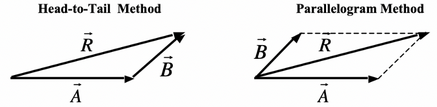
\includegraphics{img/vector-addition-methods.png}

\hypertarget{vector-subtraction}{%
\subsubsection{Vector Subtraction}\label{vector-subtraction}}

\begin{itemize}
\tightlist
\item
  The same as vector addition, but you flip the direction of the vector
  you are subtracting
\end{itemize}

\hypertarget{components-of-vectors}{%
\subsubsection{Components of Vectors}\label{components-of-vectors}}

\begin{itemize}
\tightlist
\item
  You can easily break down 2D vectors into their \(x\) and \(y\)
  components

  \begin{itemize}
  \tightlist
  \item
    \(\vec{V}_x = ||\vec{V}||\cos\theta\)
  \item
    \(\vec{V}_y = ||\vec{V}||\sin\theta\)
  \end{itemize}
\end{itemize}

\hypertarget{what-if-i-dont-know-theta-or-vecv}{%
\paragraph{\texorpdfstring{What if I don't know \(\theta\) or
\(||\vec{V}||\)?}{What if I don't know \textbackslash theta or \textbar\textbar\textbackslash vec\{V\}\textbar\textbar?}}\label{what-if-i-dont-know-theta-or-vecv}}

Well, you can easily figure that out with some trig:

\begin{itemize}
\tightlist
\item
  \(||\vec{V}|| = \sqrt{\vec{V}_x^2 + \vec{V}_y^2}\)
\item
  \(\theta = \tan^{-1}\left(\frac{\vec{V}_y}{\vec{V}_x}\right)\)
\end{itemize}

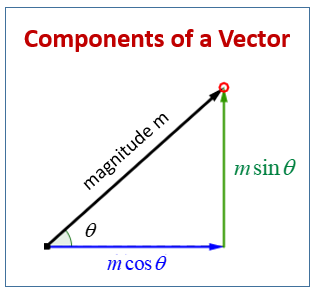
\includegraphics{img/components-vector.png}

\hypertarget{unit-vectors}{%
\subsubsection{Unit Vectors}\label{unit-vectors}}

\begin{itemize}
\tightlist
\item
  A \textbf{unit vector} is any vector with a magnitude of 1
\item
  If you take the vector (cross) product of the unit vectors in the
  \(x\) and \(y\) direction, the resultant vector will be the same in
  the \(z\) direction

  \begin{itemize}
  \tightlist
  \item
    \(\hat{i} \times \hat{j} = \hat{k}\)
  \end{itemize}
\end{itemize}

\hypertarget{unit-vector-notation}{%
\subsubsection{Unit Vector Notation}\label{unit-vector-notation}}

\begin{itemize}
\tightlist
\item
  You can represent a vector in unit vector notation by multiplying the
  unit vectors by their respective components:

  \begin{itemize}
  \tightlist
  \item
    \(\vec{V} = V_x\hat{i} + V_y\hat{j} + V_z\hat{k}\)
  \end{itemize}
\item
  You can also add two vectors in unit vector notation as follows:

  \begin{itemize}
  \tightlist
  \item
    \(\vec{V} + \vec{W} = (V_x + W_x)\hat{i} + (V_y + W_y)\hat{j} + (V_z + W_z)\hat{k}\)
  \end{itemize}
\item
  You can also represent a vector in unit vector notation by multiplying
  the unit vectors by their respective magnitudes and the cosine of the
  angle between the vector and the unit vector

  \begin{itemize}
  \tightlist
  \item
    For example:
    \(\vec{V} = ||\vec{V}||\cos\theta\hat{i} + ||\vec{V}||\cos\theta\hat{j} + ||\vec{V}||\cos\theta\hat{k}\)
  \end{itemize}
\end{itemize}

\hypertarget{unit-vectors-to-find-position}{%
\subsubsection{Unit Vectors to Find
Position}\label{unit-vectors-to-find-position}}

You can use unit vectors to find the position of a vector:
\begin{align*}
\vec{r} &= r_x\hat{i} + r_y\hat{j} + r_z\hat{k} \\
\vec{v} &= \frac{\mathrm{d}\vec{r}}{\mathrm{d}{t}} = \frac{\mathrm{d}}{\mathrm{d}{t}}(r_x\hat{i}) + \frac{\mathrm{d}}{\mathrm{d}{t}}(r_y\hat{j}) + \frac{\mathrm{d}}{\mathrm{d}{t}}(r_z\hat{k}) \\
&= \frac{\mathrm{d}r_x}{\mathrm{d}t}\hat{i} + \frac{\mathrm{d}r_y}{\mathrm{d}t}\hat{j} + \frac{\mathrm{d}r_z}{\mathrm{d}t}\hat{k} \\
\end{align*}

\hypertarget{why-does-this-work}{%
\paragraph{Why does this work?}\label{why-does-this-work}}

Remember that the derivative of a constant is 0, and
\(\hat{i}, \hat{j}, \hat{k}\) are constants: \begin{align*}
\frac{\mathrm{d}}{\mathrm{d}t}(r_x\hat{i}) = \frac{\mathrm{d}r_x}{\mathrm{d}t}\hat{i} + r_x\frac{\mathrm{d}\hat{i}}{\mathrm{d}t}
\end{align*}



\end{document}
